\chapter{Descrição da fonte e caracterização do conjunto de dados}
\label{cap:dados}

\section{Fonte e variáveis}
\label{sec:entradas}

Foi utilizado o conjunto \textit{Acidentes nas Rodovias Federais (agrupados por ocorrência)}, publicado pela PRF no Portal Brasileiro de Dados Abertos \cite{prf2026}: um arquivo CSV por ano, de 2007 a 2026, com uma linha por acidente, somando 2.237.189 registros. As 12 entradas, todas categóricas, estão no Quadro~\ref{qua:entradas}, em três grupos. As contagens de pessoas e veículos têm caudas longas (mediana 2, mas até 248 pessoas e 131 veículos num registro) e foram convertidas em faixas, que é também o que um solicitante consegue informar.

\begin{quadro}[!htbp]
\caption{Variáveis de entrada}
\label{qua:entradas}
\begin{center}
\footnotesize
\begin{tabularx}{\textwidth}{|P{1.7cm}|l|P{1.45cm}|P{2.9cm}|Y|}
\hline
\textbf{Grupo} & \textbf{Variável} & \textbf{Categorias} & \textbf{Mais frequente} & \textbf{Observação} \\ \hline
\multirow{4}{1.7cm}{Contexto da via}
 & \texttt{condicao\_metereologica} & 10 & céu claro (52\%) & \texttt{ignorado} mantido como valor legítimo \\ \cline{2-5}
 & \texttt{tipo\_pista} & 3 & simples (52\%) & simples, dupla, múltipla \\ \cline{2-5}
 & \texttt{tracado\_via} & 4 & reta (70\%) & multirrótulo desde 2017, reduzido à geometria principal \\ \cline{2-5}
 & \texttt{fase\_dia} & 4 & pleno dia (57\%) & \\ \hline
\multirow{4}{1.7cm}{Quando e onde}
 & \texttt{uf} & 27 & MG (14\%) & \\ \cline{2-5}
 & \texttt{br} & 213 (105 após agrupar raras) & 101 e 116 (17\% cada) & número da rodovia tratado como rótulo \\ \cline{2-5}
 & \texttt{fim\_de\_semana} & 2 & não (53\%) & derivada de \texttt{dia\_semana} (sexta a domingo) \\ \cline{2-5}
 & \texttt{periodo\_dia} & 4 & tarde (32\%) & derivada de \texttt{horario} (faixas de 6 h) \\ \hline
\multirow{4}{1.7cm}{Relato do solicitante}
 & \texttt{tipo\_acidente} & 19 & colisão traseira (25\%) & sinônimos entre formatos unificados \\ \cline{2-5}
 & \texttt{macro\_causa} & 7 & desatenção\slash manobra (44\%) & agrupa as até 75 causas detalhadas \\ \cline{2-5}
 & \texttt{veiculos\_cat} & 4 & 2 (51\%) & faixas 1, 2, 3, 4+ \\ \cline{2-5}
 & \texttt{pessoas\_cat} & 5 & 2 (48\%) & faixas 1, 2, 3, 4, 5+ \\ \hline
\end{tabularx}
\end{center}
\fontequa{Elaborado pelo autor}
\end{quadro}

\section{Qualidade dos dados e distribuição do alvo}
\label{sec:alvo}

A base tem poucos problemas: no máximo 70 ausentes por coluna de entrada, 11.697 linhas (0,52\%) com alvo ausente ou \texttt{Ignorado} e 6 duplicatas exatas; o \texttt{id} se repete entre anos e foi ignorado. As contagens de vítimas são coerentes com o rótulo (todo \texttt{Com Vítimas Fatais} tem mortos $>$ 0), e os 1.081 acidentes com 10 ou mais veículos são engavetamentos plausíveis, absorvidos pela faixa \texttt{4+}. Foram removidas 11.875 linhas (0,53\%), restando 2.225.314 acidentes.

O alvo é desbalanceado (Figura~\ref{fig:alvo}): \texttt{Com Vítimas Feridas} 48,4\%, \texttt{Sem Vítimas} 46,7\% e \texttt{Com Vítimas Fatais} 4,9\%. A fração de \texttt{Sem Vítimas} cai de cerca de 60\% até 2014 para cerca de 16\% a partir de 2019: uma mudança no procedimento de registro, não no perfil dos acidentes.

\begin{figure}[!htbp]
  \centering
  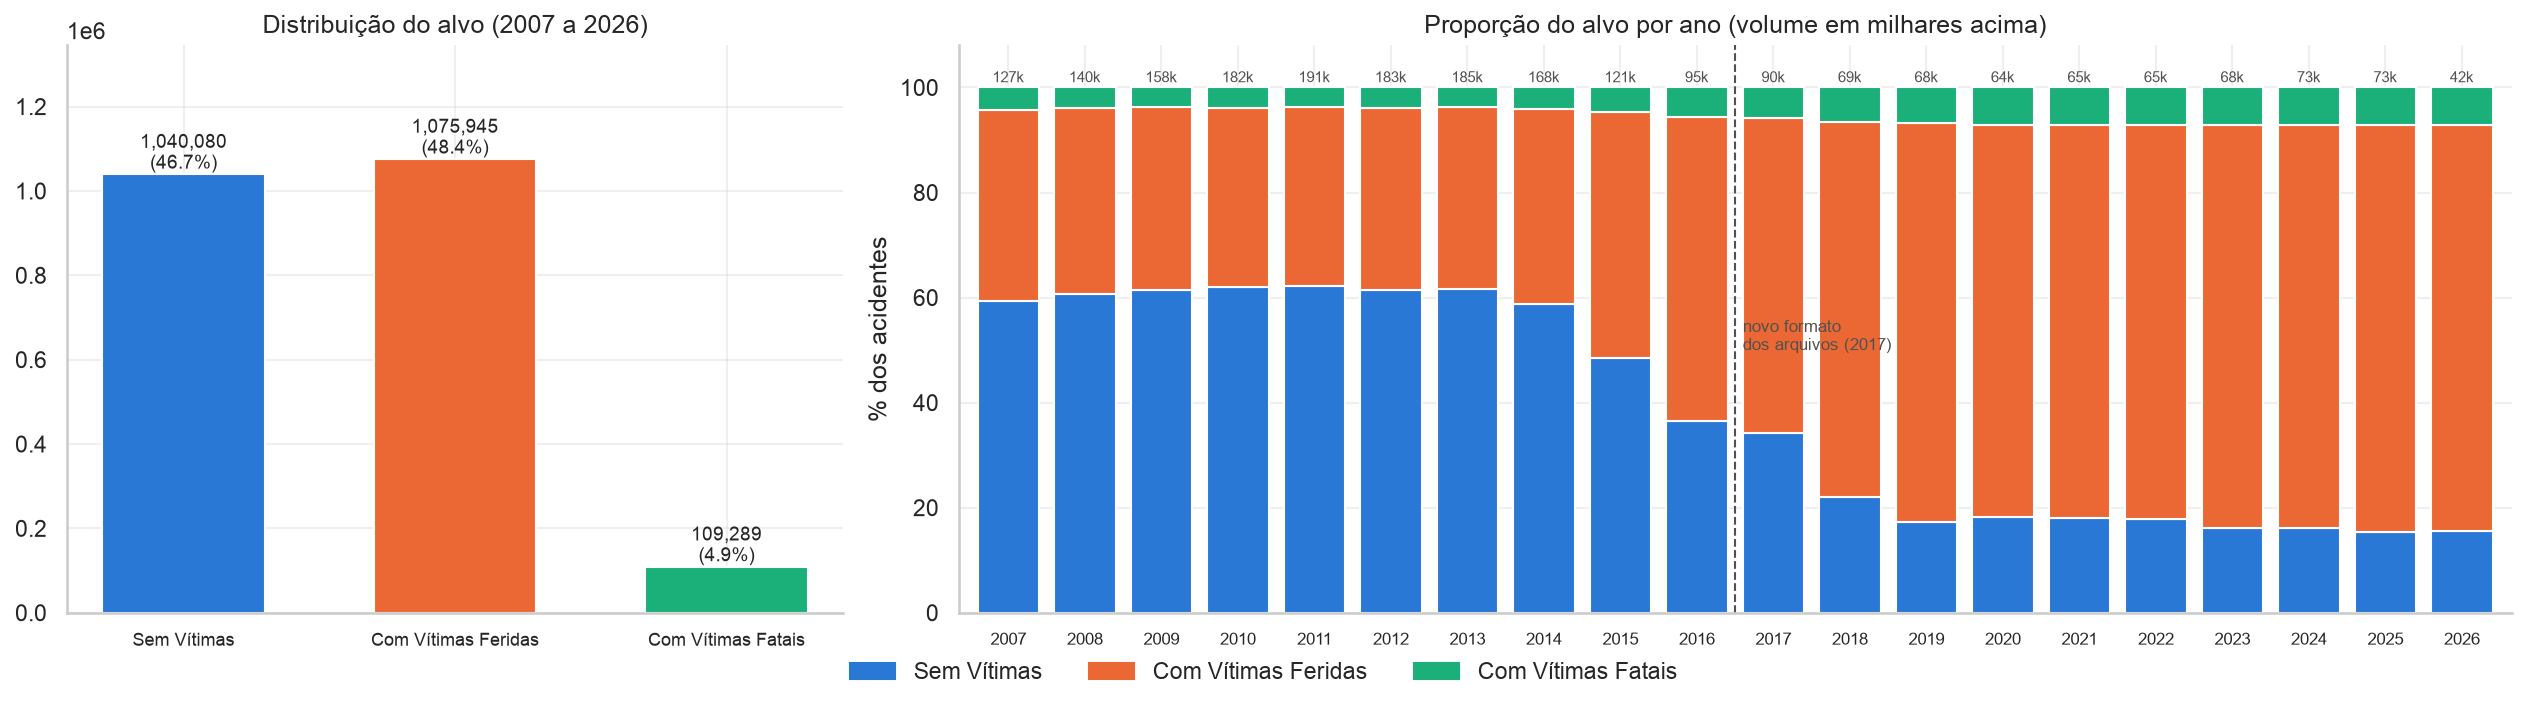
\includegraphics[width=0.7\textwidth]{figuras/01_alvo}
  \caption{Distribuição do alvo e proporção por ano}
  \label{fig:alvo}
  \fontefig{Elaborado pelo autor}
\end{figure}

A hora e o dia da semana importam (Figura~\ref{fig:hora-dia}): a taxa de fatais chega a 9\% na madrugada, contra cerca de 3\% entre 7 h e 17 h, e sobe no sábado (5,8\%) e no domingo (6,7\%), contra cerca de 4,3\% nos demais dias. Isso motivou derivar \texttt{periodo\_dia} e \texttt{fim\_de\_semana} (esta última agrupando sexta, sábado e domingo, os dias de maior volume). A mesma figura, à direita, compara, para cada entrada, a taxa de fatais da categoria mais letal com a da menos letal: as variáveis do relato do solicitante separam muito mais (27,9 p.p. em \texttt{tipo\_acidente}) que as de contexto da via (4 a 5 p.p.).

\begin{figure}[!htbp]
  \centering
  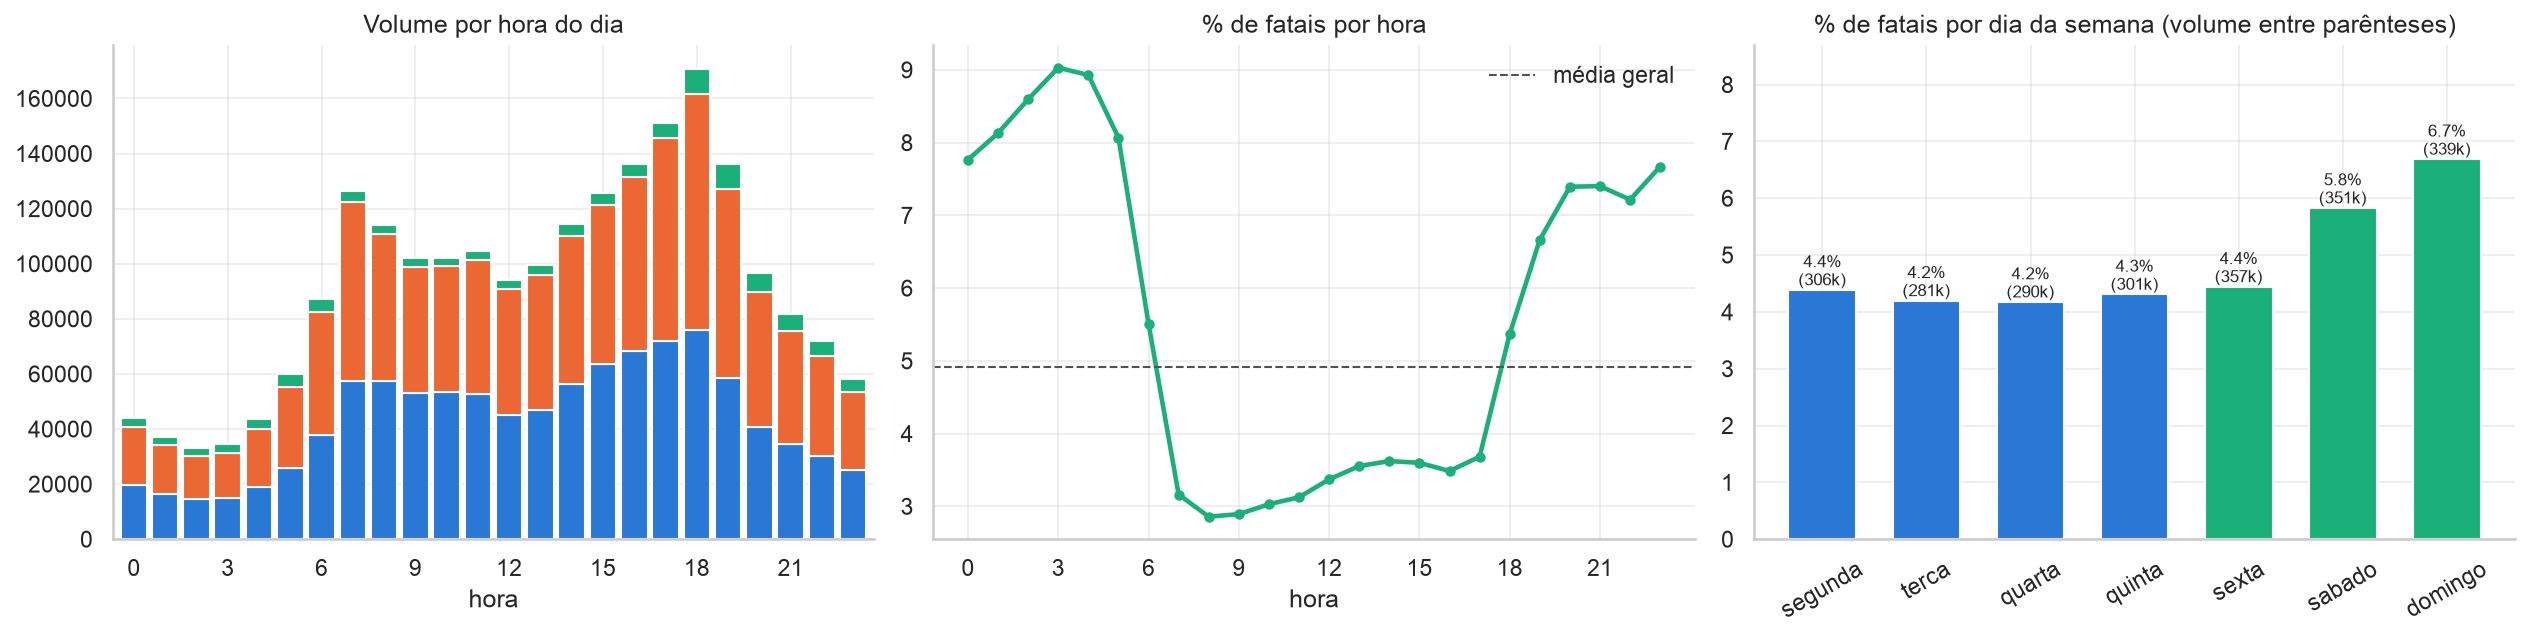
\includegraphics[width=0.6\textwidth]{figuras/02_hora_dia_semana}\hfill
  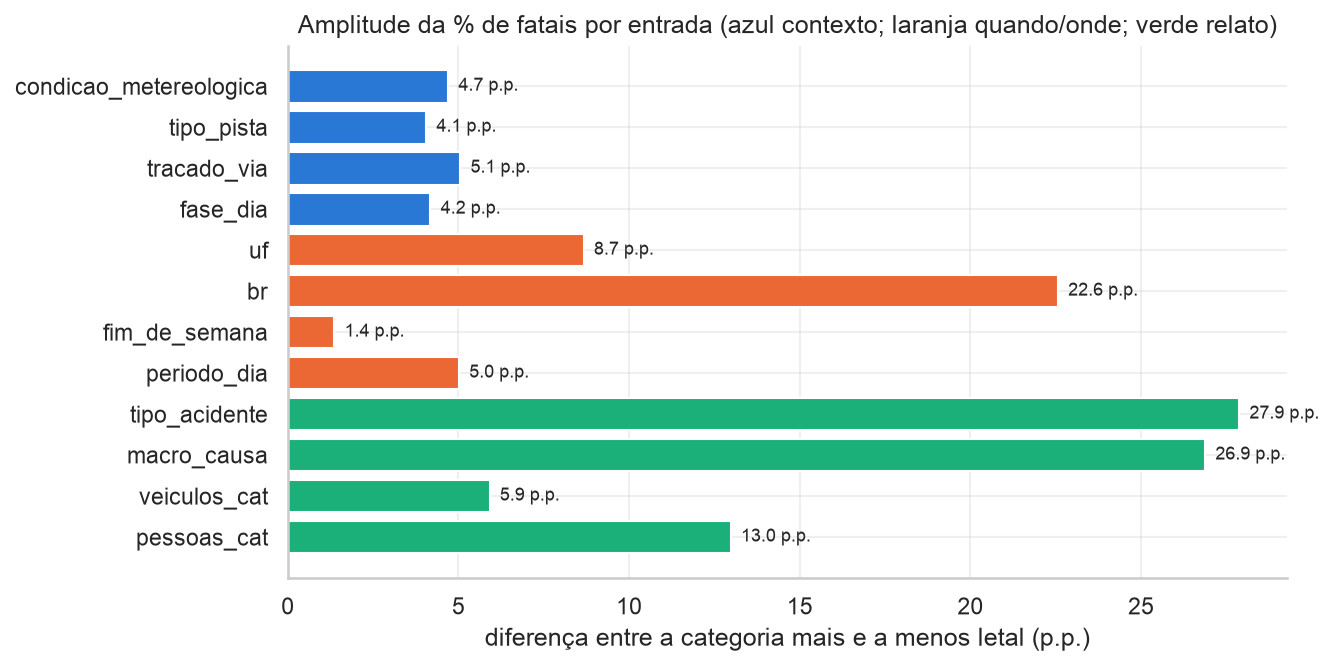
\includegraphics[width=0.38\textwidth]{figuras/09_amplitude_fatais}
  \caption{À esquerda, volume por hora e taxa de fatais por hora e por dia da semana; à direita, amplitude da taxa de fatais por entrada}
  \label{fig:hora-dia}
  \fontefig{Elaborado pelo autor}
\end{figure}

\section{Seleção de atributos e risco de vazamento}
\label{sec:selecao}

As contagens de vítimas (\texttt{mortos}, \texttt{feridos}, \texttt{ilesos} etc.) definem o rótulo e foram excluídas: seriam vazamento direto. Para que o modelo não aprendesse o período de registro em vez da gravidade, saíram também o \texttt{ano} e os campos que só existem a partir de 2017 (coordenadas, \texttt{regional}, \texttt{delegacia}, \texttt{uop}), e a causa detalhada, cujo vocabulário cresce de 11 valores em 2016 para 75 em 2023, foi agrupada em 7 macrocausas. \texttt{km}, \texttt{municipio} e \texttt{sentido\_via} saíram por cardinalidade alta ou pouca informação depois de \texttt{uf} e \texttt{br}. \texttt{causa\_acidente} é avaliação da equipe, não do solicitante, e pode não existir na triagem; seu efeito isolado não foi medido (Capítulo~\ref{cap:conclusao}).

\section{Divisão dos dados e pré-processamento}
\label{sec:preproc}

Os dados foram divididos em 70\% treino (1,56 milhão), 15\% validação (334 mil) e 15\% teste (334 mil), com estratificação pelo alvo. A divisão é aleatória porque não há unidades com várias observações, mas mistura no teste os dois regimes de registro da Seção~\ref{sec:alvo}: a estimativa vale para a distribuição histórica, não para o uso futuro. A validação cruzada não foi usada pelo custo com 2,2 milhões de linhas. O teste não participa de nenhuma seleção.

As entradas foram codificadas com \texttt{OneHotEncoder} ajustado somente no treino; categorias com menos de 200 ocorrências ou nunca vistas vão para uma coluna \aspas{infrequente}. O resultado são 194 colunas binárias, sem necessidade de normalização. Para o desbalanceamento, a perda recebe pesos de classe calculados no treino, com raiz quadrada aplicada (0,845 / 0,830 / 2,605): o peso integral ($\approx$6,8 para fatais) faria o modelo prever fatal em excesso. O expoente 0,5 foi fixado, não buscado, e define o ponto de operação entre \textit{recall} e precisão dos fatais.
